\chapter{Processing text}
\label{chap:protext}


\begin{abstract}{Abstract}
Many datasets that are relevant for social science consist of textual data, from political discussions and newspaper archives to open-ended survey questions and reviews. This chapter gives an introduction to dealing with textual data using base functions in Python and (mostly) the \index{stringr}\emph{stringr} package in R.
\end{abstract}

\keywords{Text representation, text cleaning, regular expressions}

\begin{objectives}
\item Understand how text is represented in the computer
\item Be able to clean up and alter text
\item Understand and be able to use regular expressions
\end{objectives}


\newpage
\begin{feature}
  \textbf{Packages used in this chapter}\\
  This chapter introduces the packages for handling textual data.
  For R, this is mainly the \index{stringr}\emph{stringr} package (included in \index{tidyverse}\emph{tidyverse}).
  In Python, most functions are built-in, but will show how to use these functions in \index{pandas}\emph{pandas} and also introduce the \index{regex}\emph{regex} alternative to built-in regular expressions.
You can install these packages with the code below if needed  (see Section~\ref{sec:installing} for more details):

\doublecodex{chapter10/chapter10install}

\noindent After installing, you need to import (activate) the packages every session:

\doublecodex{chapter10/chapter10library}

\end{feature}

%\section{Reading and cleaning text}
\label{sec:readtext}

When dealing with textual data, an important step is to normalize the data. Such preprocessing ensures that noise is removed, and reduces the amount of data to deal with. In \refsec{encodings} we explained how to read data from different formats, such as txt, csv or json that can include textual data, and we also mentioned some of the challenges when reading text (i.e. encoding/decoding from/to Unicode). In this section we cover typical cleaning steps such as lowercasing and removing punctuation, HTML tags and boilerplate.
 
As a computational communication scientist you will come across with many sources of text that range from electronic versions of newspapers in HTML to parliamentary speeches in PDF. Moreover, most of the contents in their original shape will include data that will not be of interest for the analysis but, instead,  will produce noise that might negatively affect the quality of the research. You have to decide which parts of the raw text should be considered for analysis and determine the shape of these contents in order to have a good input in the analytical process. 

There is not a rule of thumb that can guide you in this preprocessing stage, and it is highly likely that you will have to test different combination of steps and assess what are the best options. For example, in some cases keeping capital letters within a chat conversation or a news comment might be valuable to detect the tone of the message, but in more formal speeches transforming the whole text to lowercases would help to normalize the content. However, it is true that there some typical challenges to reduce the noise from the text.

The first thing to keep in mind is that once you load any text on R or Python you usually store this content as a \emph{character} or \emph{string} object (or you may also think of \emph{lists} or \emph{dictionaries}, but they will have strings inside anyway), which means that basic operations and conditions of this data type apply, such as indexing or slicing to access individual characters or substrings (see \refsec{datatypes}). In fact, base strings operations are very powerful to clean your text and eliminate a big amount of noise of it.  Table~\ref{tab:stringoperations} summarises some useful operations on strings in R and Python that will help you in this stage.   

\begin{table}
  \caption{\label{tab:stringoperations}Useful strings operations in R and Python to clean noise}{
  \begin{tabularx}{\textwidth}{lllll}
    \toprule
String operation      & R   & Python\\ \midrule
Count characters      & nchar(string) & len(string)  \\
Get a substring       & substr(string, start=n1, stop=n2) & string[n1:n2]            \\
Split the string into several strings   & strsplit(string, split) & split(string, split)             \\ 
Convert to lowercase  & tolower(string) & string.lower     \\ 
Convert to uppercase  & toupper(string) & string.upper     \\ 
Find and replace      & gsub("substring1","substring2",string) & string.replace('substring1','substring2') \\ 
    \bottomrule
  \end{tabularx}}{}
\end{table}

Let us apply some of these functions/methods to a simple Wikipedia text that contains HTML tags or boilerplate, punctuation and natural upper/lower case letters. Using base function \fn{gsub} in R and \fn{replace} in Python we can remove strings containing specific expressions such as \texttt{<p>} or \texttt{</b>} and include an empty space instead. We can use this same method to eliminate punctuation taking as a reference a pre-defined list of signs (\texttt{:punct:} in base R or the object \texttt{punctuation} from the library \pkg{string} in Python). In the case of converting letters from upper to lower case, we use the base R function \fn{tolower} and the string method \fn{lower} in Python. To remove unnecessary double spaces we apply the base R function \fn{trimws} and method \fn{join} in Python. \refex{clean} shows how to conduct this cleaning process.

\pyrex[output=both,caption=Cleaning text with base functions]{chapter10/clean}

It is good news that we have some extra packages that facilitate this initial stage and clean boilerplate. For instance, you can think of \pkg{stringi} in R (recommended by \citet{welbers2017text} as a better option than built-it functions) or \pkg{Beautiful Soup} in Python. \refex{cleanextra} shows how to implement these packages to remove html tags.

\pyrex[output=both,caption=Cleaning text with stringi and Beautiful Soup]{chapter10/cleanextra}

As you can notice in the R example, the package \pkg{stringi} removed the tags using the function \fn{stri\_replace\_all} and a \emph{regular expression} (which are very useful in this cleaning stage and that we will explain in the next section). We also eliminated the surrounding white spaces with the function \fn{stri\_trim}. In the case of the Python example, the library \pkg{BeautifulSoup} helps you to \emph{parse} the text with the same-name function \fn{BeautifulSoup} and then extract the text without the html tags using the function \fn{get\_text}.	

When dealing with textual data, an important step is to normalize the data. Such preprocessing ensures that noise is removed, and reduces the amount of data to deal with. In Section~\ref{sec:encodings} we explained how to read data from different formats, such as txt, csv or json that can include textual data, and we also mentioned some of the challenges when reading text (i.e.\ encoding/decoding from/to Unicode). In this section we cover typical cleaning steps such as lowercasing and removing punctuation, HTML tags and boilerplate.

As a computational communication scientist you will come across many sources of text that range from electronic versions of newspapers in HTML to parliamentary speeches in PDF. Moreover, most of the contents in their original shape will include data that will not be of interest for the analysis but, instead,  will produce noise that might negatively affect the quality of the research. You have to decide which parts of the raw text should be considered for analysis and determine the shape of these contents in order to have a good input in the analytical process.

As the difference between useful information and noise is determined by your research question,
there is not a fixed list of steps to take that can guide you in this preprocessing stage.
It is highly likely that you will have to test different combinations of steps and assess what  the best options are.
For example, in some cases keeping capital letters within a chat conversation or a news comment might be valuable to detect the tone of the message, but in more formal speeches transforming the whole text to lowercases would help to normalize the content.
However, it is true that there are some typical challenges to reducing the noise from the text.

This chapter and the next will show you how to clean and manipulate text to transform the raw strings of letters into useful data.
This chapter focuses on dealing with the text as characters and especially shows you how to use \index{regular expressions}\emph{regular expressions} to search and replace textual content.
The next chapter will focus on text as words and shows how you can represent text in a suitable format for further computational analysis.

\section{Text as a String of Characters} \label{sec:unicode}

\note{\textbf{Important: Unicode and Encodings}
  Technically speaking, text is represented as bytes (numbers) rather than characters.
  The  Unicode standard determines how these bytes should be interpreted or ``decoded''.
  This chapter assumes that the bytes in a file are already ``decoded'' into characters (or Unicode code points),
  and we can just work with the characters.
  Especially if you are not working with English text, it is very important to make sure you understand Unicode and encodings
  and check that the texts you work with are decoded properly.
  Please see Section~\ref{sec:encodings} for more information on how this works.}

When we think about text, we might think sentences or words, but the computer only ``thinks'' about letters:
text is represented internally as a string of characters.
This is reflected of course in the type name, with R calling it a \index{character}\emph{character} vector and Python a \index{string}\emph{string}.

\begin{ccsexample}
  \begin{center} 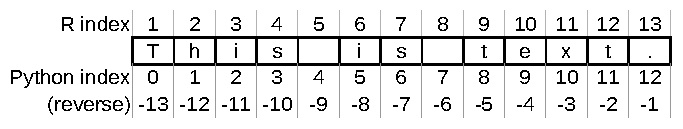
\includegraphics[width=.6\textwidth]{chapter09/text.pdf}\end{center}

\doublecodex{chapter10/string}
\doubleoutput{chapter10/string}
\doublecodex{chapter10/manystrings}
\doubleoutput{chapter10/manystrings}

  \caption{Internal representation and of single and multiple texts.}\label{ex:text}
\end{ccsexample}

As a simple example, the figure at the top of Example~\ref{ex:text} shows how the text ``This is a text.'' is represented.
This text is split info separate characters, with each character representing a letter (or space,  punctuation, emoji, or Chinese character).
These characters are indexed starting from the first one, with (as always) R counting from one, but Python counting from zero.

In Python, texts are represented as \index{str}\texttt{str} (string) objects, in which we can directly address the individual characters by their position: \texttt{\small{text[0]}} is the first character of \texttt{\small{text}}, and so on.
In R, however, texts (like all objects) represent columns (or vectors) rather than individual values.
Thus, \texttt{\small{text[1]}} in R is the first text in a series of text.
To access individual characters in a text, you have to use a function such as \index{str\_length}\texttt{str\_length} and \index{str\_sub}\texttt{str\_sub} that will be discussed in more detail below.
This also means that in Python, if you have a column (or list) of strings that you need to apply an operation to,
you either need to use one of Panda's methods shown below or use a \index{for loop}\emph{for loop} or \index{list comprehension}\emph{list comprehension} to iterate over all the strings.

\subsection{Methods for Dealing With Text}

\note{\textbf{Stringi, stringr, and base string operations in R}
  As is so often the case, R has multiple packages that partially replicate functionality for basic text handling.
  In this book we will mainly use the \index{stringr}\emph{stringr} package, which is part of \index{tidyverse}\emph{tidyverse}.
  This is not because that package is necessarily better or easier than the alternative \index{stringi}\emph{stringi} package
  or the built-in (\index{base}\emph{base}) methods.
  However, the methods are well-documented, clearly named, and consistent with other tidyverse functions,
  so for now it is easiest to stick to \index{stringr}\emph{stringr}.
  In particular, \index{stringr}\emph{stringr} is very similar to \index{stringi}\emph{stringi} (and in fact is partially based on it).
  So, to give one example, the function \index{str\_detect}\texttt{str\_detect} is more or less the same as \index{stringi::str\_detect}\texttt{stringi::str\_detect} and \index{base::grepl}\texttt{base::grepl}.
}

The first thing to keep in mind is that once you load any text on R or Python you usually store this content as a \emph{character} or \emph{string} object (you may also often use \emph{lists} or \emph{dictionaries}, but they will have strings inside then), which means that basic operations and conditions of this data type apply, such as indexing or slicing to access individual characters or substrings (see Section~\ref{sec:datatypes}). In fact, base strings operations are very powerful to clean your text and eliminate a large amount of noise.  Table~\ref{tab:stringoperations} summarizes some useful operations on strings in R and Python that will help you in this stage.

\begin{table}
  \caption{\label{tab:stringoperations}Useful strings operations in R and Python to clean noise.}{
  \begin{tabularx}{\textwidth}{lllll}
    \toprule
    String operation      & R (\index{stringr}\emph{stringr})  & Python  & Pandas\\
                          & (whole column)  & (single string) & (whole column)\\
    \midrule
Count characters in s & \texttt{\small{str\_length(s)}}          & \texttt{\small{len(s)}}        & \texttt{\small{s.str.len()}}  \\
Extract a substring   & \texttt{\small{str\_sub(s, n1, n2)}}     & \texttt{\small{s[n1:n2]}} & \texttt{\small{s.str.slice(n1, n2)}} \\
Test if s contains s2 & \texttt{\small{str\_detect(s, s2)}}$^*$       & \texttt{\small{s2 in s}}       & \texttt{\small{s.str.match(s2)$^*$}} \\
Strip spaces          & \texttt{\small{trimws(s)}}               & \texttt{\small{s.strip()}}     & \texttt{\small{s.str.strip()}} \\
Convert to lowercase  & \texttt{\small{tolower(s)}}              & \texttt{\small{s.lower()}}     & \texttt{\small{s.str.upper()}} \\
Convert to uppercase  & \texttt{\small{toupper(s)}}              & \texttt{\small{s.upper()}}     & \texttt{\small{s.str.lower()}} \\
Find s1 and replace by s2 & \texttt{\small{str\_replace(s, s1, s2)}}$^*$ & \texttt{\small{s.replace(s1, s2)}} & \texttt{\small{s.str.replace(s1, s2)$^*$}}  \\
    \bottomrule
  \end{tabularx}}{(*) The R functions \texttt{\small{str\_detect}} and \texttt{\small{str\_replace}} and the Pandas function \texttt{\small{s.str.match}} and \texttt{\small{s.str.replace}} use \index{regular expressions}\emph{regular expressions} to define what to find and replace. See Section~\ref{sec:regular} below for more information.}
\end{table}

Let us apply some of these functions/methods to a simple Wikipedia
text that contains HTML tags or boilerplate and natural upper/lower
case letters.
Using the \index{stringr}\emph{stringr} function \index{str\_replace\_all}\texttt{str\_replace\_all} in R
and \index{replace}\texttt{replace} in Python we can do a find-and-replace and replace substrings
by others (in our case, replace \texttt{<b>} with a space, for instance).
To remove unnecessary double spaces we apply the \index{str\_squish}\texttt{str\_squish} function provided by \index{stringr}\emph{stringr} and in Python,
we first chunk our string into a list of words by using the \index{split}\texttt{split} string method, before we use the \index{join}\texttt{join} method
to join them again with now a single space.
In the case of converting letters from upper to lower case, we use the base R function \index{tolower}\texttt{tolower} and the string
method \index{lower}\texttt{lower} in Python.
Finally, the base R function \index{trimws}\texttt{trimws} and the
Python string method \index{strip}\texttt{strip} remove the white space from the beginning
and end of the string.
Example~\ref{ex:clean} shows how to conduct this cleaning process.

While you can get quite far with these techniques, there are more advanced and flexible approaches possible.
For instance, you probably do not want to list \emph{all possible} HTML tags in separate \index{replace}\texttt{replace} methods or \index{str\_replace\_all}\texttt{str\_replace\_all} functions. In the next section, we therefore show how to use so-called \index{regular expressions}\emph{regular expressions} to formulate such generalizable patterns.

\pyrex[output=both,caption=Some basic text cleaning approaches]{chapter10/clean}

\note{\textbf{To regex or not to regex in Python} You may wonder why we introduce basic string methods like \index{replace}\texttt{replace} or the \index{split}\texttt{split}-then-\index{join}\texttt{join} trick, if everything can be done with regular expressions anyway. There are a couple of reasons for still using these methods: first, they are easy and don't have any dependencies. If you just want to replace a single thing, then you don't need to import any additional module. Second, regular expressions are considerably slower than string methods -- in most cases, you won't notice, but if you do a lot of replacements (think in thousands per news article, for a million  articles), then this may matter. Third, you can use the \index{join}\texttt{join} trick also for other things like punctuation removal -- in this case, by generating a list of all characters in a string called \verb|text| provided they are no punctuation characters, and then joining them directly to each other:
\verb|from string import punctuation; "".join([c for c in text if c not in punctuation])|}


%\section{Regular expressions}
\label{sec:regular}

A \concept{regular expression} or \emph{regex} is a powerful language to locate strings that conform a given pattern. For instance, we can extract usernames or email-addresses from text, or normalize spelling variations and improve the cleaning methods covered in the previous section. Specifically, regular expressions are a sequence of characters that we can use to design a pattern and then use this pattern to \emph{find} strings (identify or extract) and also \emph{replace} those strings by new ones. 

Regular expressions look complicated, and in fact they take some getting used to initially.
For example, a relatively simple (and not quite correct) expression to match an email address is \verb|[\w\.-]+@[\w\.-]+\.\w\w+|,
which doesn't look like anything at all unless you know what you are looking for.
The good news is that regular express syntax is the same in R and Python (and many other languages),
so once you learn regular expressions you will have acquried a powerful and versatile tool for text processing. 

%We will show how you can use regexes to preprocess text. The good thing is that regular expression syntax can be similar in R and Python and once you learn how to write a pattern in one language it is easy to do the same in the other.  However they are not identical! Even it is out of the scope of this book, you can trace the specific standards of each language and its different versions. You will come across with some standards of the Portable Operating System Interface (POSIX), such as the Basic Regular Expressions (BRE) or Extended Regular Expressions (ERE), or also with the Perl Compatible Regular Expressions (PCRE).  By default the R function \fn{grep} uses ERE but you can set a parameter (\verb|perl = TRUE|) to work with PCRE, and in the case of Python \fn{re} module regexes match operations similar to PCRE as a default.

%% \note{\textbf{Python: re versus regex}
%%   In python, people generally use the \pkg{re} package for regular expressions.
%%   In this book we will use the \pkg{regex} package, however.
%%   This modules has the same functions and arguments as the \pkg{re} module,
%%   but it has better support for unicode, which is very important when dealing with non-western text.
%%   However, for almost all examples you can also use the \pkg{re} module if prefered.
%%   }

In the next section, we will first review general expression syntax without reference to running them in Python or R.
Subsequently, you will see how you can apply these expression to inspect and clean texts in both languages.

\subsection{Regular expression syntax}

At its core, regular expressions are patters for matching sequences of characters.
In the simplest case, a regular letter just matches that letter, so the pattern `cat' matches the text `cat'.
Next, there are various wildcards, or ways to match different letters.
For example, the period (\verb|.|) matches any character, so \verb|c.t| matches both `cat' and `cot'.
You can place mulitple letters between square brackets to create a \concept{character class} that matches all the specified letters, so \verb|c[au]t| matches `cat' and `cut', but not `cot'.
There are also a number of pre-defined classes, such as \verb|\w| which matches `word characters' (letters, digits, and (curiously) underscores).

Finally, for each character or group of characters you can specify how often it should occur.
For example, \verb|a+| means one or more a's while \verb|a?| means zero or one a, so \verb|lo+l| matches `lol', `lool', etc.,
and \verb|lo?l| matches `lol' or `ll'.
This raises the question, of course, of how to look for actual occurrences of a plus, question mark, or period.
The solution is to \concept{escape} these special symbols by placing a backslash (\verb|\|) before them:
\verb|a\+| matches the literal text `a+', and \verb|\\w| (with a double backslash) matches the literal text `\textbackslash w'. 

Now, we can have another look at the example emails address pattern given above.
The first part, \verb|[\w\.-]| creates a character class containing word characters, (literal) periods, and dashes.
Thus, \verb|[\w\.-]+@[\w\.-]+| means one or more letters, digits, underscores, periods, or dashes, followed by an at sign,
followed by one or more letters, digits, etc.
Finally, the last part \verb|\.\w\w+| means a literal period, a word character, and one or more word characters.
In other words, we are looking for a name (possibly contining dashes or periods) before the at sign,
followed by a domain, followed by a top level domain (like \verb|.com|) of at least two characters.

In essence, thinking in terms of what you want to match and how often
you want to match it is all there is to regular expressions.
However, it will take some practice to get comfortable with turning something sensible (such as an email address) into a correct regular expression pattern.
The next subsection will explain regular expression syntax in more detail, followed by an explanation of grouping,
and in the final subsection we will see how to use these regular expressions in R and Python to do text cleaning. 

\newcommand{\fnregexnote}{\footnote{Note that this is not a full review of everything that is possible with regular expressions, but this includes the most used options and should be enough for the majority of cases. Moreover, if you descend into the more specialized aspects of regular expressions (with beautiful names such as `negative lookbehind assertions') you will also run into differences between Python, R, and other languages, while the features used in this chapter should function in most implementations you come across unless specifically noted.}}




\newcommand{\ttt}[1]{\texttt{\small{#1}}}
\newcommand{\bs}[1]{\ttt{\textbackslash#1}}

\begin{table}
  \caption{\label{tab:regex}Regular expression syntax}{
  \begin{tabularx}{\textwidth}{lllll}
    \toprule
\multicolumn{2}{l}{Function}      & Syntax   & Example & Matches    \\
    \midrule
\multicolumn{2}{l}{\textit{What to match}} \\
& All characters except for new lines   & \ttt{.} & \ttt{d.g} & \ttt{d\textbf{i}g}, \ttt{d\textbf{!}g}\\
& Word characters$^*$
  (letters, digits, \_)         & \bs{w} & \ttt{d\textbackslash{}wg} & \ttt{dig}, \ttt{dog} \\
%& Everything except word characters     & \bs{W} \\
& Digits$^*$ (0 to 9)                       & \bs{d} & \ttt{202\textbackslash{}d} & \ttt{2020}, \ttt{2021} \\
%& Everything except digits              & \bs{D} \\
& Whitespace$^*$ (space, tab, newline) & \bs{s} \\
%& Everything except whitespace	& \bs{S} \\
& Newline	& \bs{n} & \\

& Beginning of the string	& \ttt{\^{}} & \ttt{\^{}go} & \ttt{\textbf{go} {\color{gray}go go}}\\
& Ending of the string   & \ttt{\$} & \ttt{go\$} & \ttt{{\color{gray}go go} \textbf{go}} \\
& Beginning or end of word & \bs{b} & \ttt{\textbackslash{}bword\textbackslash{}b} & \ttt{{\color{gray}a} \textbf{word}\color{gray}!} \\
& Either first or second option  & \ttt{$\cdots$\textbar$\cdots$} & \ttt{cat\textbar{}dog} & \ttt{cat}, \ttt{dog}\\

\multicolumn{2}{l}{\textit{How many to match}} \\
& Zero or more & \ttt{*} & \ttt{d.*g} & \ttt{dg}, \ttt{drag}, \ttt{d = g} \\
& Zero or more (non-greedy) & \ttt{*?} & \ttt{d.*?g} & \ttt{\textbf{dog}{\color{gray}g}} \\
& One or more & \ttt{+}  & \ttt{\textbackslash{}d+\%} & \ttt{1\%}, \ttt{200\%} \\
& One or more (non-greedy) & \ttt{+?}  & \ttt{\textbackslash{}d+\%} & \ttt{{\color{gray}20}\textbf{0\%}} \\
& Zero or one  & \ttt{?} & \ttt{colou?r} & \ttt{color}, \ttt{colour} \\
& Exactly n times  & \ttt{\{n\}} & \ttt{\textbackslash{}d{\{4\}}} & \ttt{1940}, \ttt{2020} \\
& At least n times  & \ttt{\{n,\}} \\
& Between n and m times  & \ttt{\{n,m\}} \\

\multicolumn{2}{l}{\textit{Other constructs}} \\
& Groups & \ttt{($\cdots$)} & \ttt{'(bla )+'} & \ttt{'blah blah blah'} \\
& Selection of characters & \ttt{\lbrack$\cdots$\rbrack} & \ttt{d\lbrack iuo\rbrack g}& \ttt{dig}, \ttt{dug}, \ttt{dog} \\
& Range of characters in selection & \ttt{\lbrack a-z\rbrack} \\
& Everything except selection & \ttt{\lbrack\^{}...\rbrack} \\
& Escape special character & \ttt{\textbackslash{}} & \ttt{3\textbackslash{}.14} & \ttt{3.14} \\

\multicolumn{4}{l}{\textit{Unicode character properties$^\dagger$}} \\
& Letters$^*$ & \multicolumn{2}{l}{\ttt{\textbackslash{}p\{LETTER\}}} & \ttt{words}, 
\includegraphics[height=1em]{chapter10/tango.pdf}\\
& Punctuation$^*$ &\multicolumn{2}{l}{ \ttt{\textbackslash{}p\{PUNCTUATION\}}} & . , : \\
& Quotation marks$^*$ & \multicolumn{2}{l}{\ttt{\textbackslash{}p\{QUOTATION MARK\}}} & ' ` " «  \\
& Emoji$^*$ & \multicolumn{2}{l}{\ttt{\textbackslash{}p\{EMOJI\}}} & 
\includegraphics[height=1em]{chapter10/emoji.pdf}  \\
& Specific scripts, e.g. Hangul$^*$& \multicolumn{2}{l}{\ttt{\textbackslash{}p\{HANG\}}} & 
\includegraphics[height=1em]{chapter10/hangul.pdf}\\

    \bottomrule
  \end{tabularx}}{\small
    $*$ These selectors can be inverted by changing it into a capital letter. Thus, \bs{W} matches everything except word characters, and \ttt{\textbackslash{}P\{PUNCTUATION\}} matches everything except punctuation\\
    $\dagger$ See \url{https://www.unicode.org/reports/tr44/\#Property\_Index} for a full list of unucode properties. Note that when using Python, these are only available if you use \pkg{regex}, which is a drop-in replacement for the more common \pkg{re}.}
\end{table}


In \reftab{regex} you will find an overview of the most important parts of regular expression syntax.\fnregexnote
The first part shows a number of common specifiers for determining what to match, e.g. letters, digits, etc.,
followed by the quantifiers available to determine how often something should be matched.
These quantifiers always follow a specifier, i.e. you first say what you're looking for, and then how many of those you need.
Note that by default quantifiers are greedy, meaning they match as many characters as possible.
For example, \verb|<.*>| will match everything between angle brackets, but if you have something like `<p>a paragraph</p>'
it will happily match everything from the first opening bracket to the last closing bracket.
By appending a question mark (\verb|?|) to the quantifier, it becomes non-greedy.
so, \verb|<.*?>| will match the individual `<p>' and `</p>' substrings. 

The third section discusses other constructs.
\concept[Capture Groups]{Groups} are formed using parentheses \verb|()| and are useful in at least three ways. 
First, by default a quantifier applies to the letter directly before it, so \verb|no+| matches `no', `nooo', etc.
If you group a number of characters you can apply a quantifier to the group. So, \verb|that's (not)? good| matches either `that's not good' or `that's good'.
Second, when using a vertical bar (\textbar) to have multiple options, you very often want to put them into a group so you can use it as part of a larger pattern.
For example, \verb!a (great|fantastic)? victory! matches either `a victory', `a great victory', or `a fantastic victory'.
Third, as will be discussed below in \refsec{regextract}, you can use groups to capture (extract) a specific part of a string, e.g. to get only the domain part of a web address. 

The other important construct are \concept{character classes}, formed using square brackets \verb|[]|.
Within a character class, you can specify a number of different characters that you want to match, using a dash (\verb|-|) to indicate a range.
You can add as many characters as you want: \verb|[A-F0-9]| matches digits and capital letters A through F.
You can also invert this selection using an initial caret: \verb|[^a-z]| matches everything except for lowercase Latin letters.
Finally, you sometimes need to match a control character  (e.g. \verb!+!, \verb|?|, \verb|\|). Since those characters have a special meaning within a regular expressing, they cannot be used directly. The solution is to add a backslash (\verb|\|) behind them to \concept{escape} them:
\verb|.| matches any character, but \verb|\.| matches an actual period. \verb|\\| matches an actual backslash.

\subsection{Example patterns}

Using the syntax explained in the previous section, we can now make patterns for common tasks in cleaning and analysing text.
\reftab{regexample} list a number of regular expressions for common tasks such as finding dates or stripping HTML artefacts.


\begin{table}
  \caption{\label{tab:regex}Regular expression syntax}{
    \begin{tabularx}{\textwidth}{lll}
      \toprule
      Goal & Pattern & Example \\
      \midrule
      URL & https?:// & \ttt{https://example.com?a=b} \\
      E-mail address & \ttt{[\textbackslash{}w\textbackslash{}.-]+@[\textbackslash{}w\textbackslash{}.-]+\textbackslash{}.\textbackslash{}w+} & \ttt{me@example.com} \\
      HTML tags & \ttt{</?\textbackslash{}w[\^{}>]+>} & \ttt{</html>} \\
      HTML Character escapes & \ttt{\&[\^{};]+;} & \ttt{\&nbsp;} \\
      US Zip Code (and zip+4) & \ttt{\textbackslash{d}\{5\}(-\textbackslash{d}\{4\})?} & \ttt{90210, 90210-1234} \\
      Dutch Postcode & \ttt{\textbackslash{d}\{4\} ?\lbrack{}A-Za-z\rbrack\{2\}} & \ttt{1015 GK} \\
      U.S. Phone number & \ttt{(\textbackslash{d}\{3\})\textbackslash{d}\{3\}-\textbackslash{d}\{4\}} & \ttt{(555) 123-4567}\\
      International phone number & \ttt{\textbackslash{}d+[\textbackslash{}d -]{6,}\textbackslash{}d+} & \ttt{+1 555-1234567}\\
      ISO Date and time & \ttt{\textbackslash{}d\{4\}-\textbackslash{}d\{2\}-\textbackslash{}d\{2\}(T\textbar{} )\textbackslash{}d\{2\}:\textbackslash{}d\{2\}:\textbackslash{}d\{2\}} & \ttt{2020-07-20T22:15} \\
      \bottomrule
      \end{tabularx}}{Please note that some of these patterns are not completely correct, and should not be used for e.g. validation in a financial system.
        a complete regular expression to match email addresses is over 400 characters long, and a complete HTML tag expression is impossible because they can contain nested escapes within attributes.
        For a better way to deal with analysing HTML, please see \refchap{scraping}. In the end, patterns like these are fine for a (somewhat) noisy analysis of (often also somewhat noisy) source texts,
        and it is fine to use such patterns as long as you understand the limitations. }
\end{table}



We start with a number of relatively simple patterns for Zip codes and phone numbers.
Starting with the simplest example, US Zip codes are simply five consecutive numbers.
Next, a US phone number can be written down as three groups of numbers separated by parentheses,
where the first group is made optional for local phone numbers using parentheses to group these numbers so the question mark applies to the whole group. 
Next, Dutch postal codes are simply 4 numbers followed by 2 letters, and we allow an optional space in between.
Similarly simple, dates in ISO format are 3 groups of numbers separated by dashes.
German dates follow a different order, use periods as separator, and allow for single-digit day and month numbers.
Note that these patterns do not check for the validity of dates.
A simple addition would be to restrict months to 01-12, e.g. using \verb!(0[1-9]|1[0-2])!.
However, in general validation is better left to specialized libraries, as properly validitaing the day number would require taking the month (and leap years) into account. 

A slightly more complicated pattern is the one given for international phone numbers.
They always start with a plus sign and contain at least 8 numbers, but can contain dashes and spaces depending on the country.
So, after the literal \verb|+| (which we need to escape since \verb|+| is a control character),
we look for 7 or more numbers, optionally followed by a single dash or space, and end with a single number.
This allows dashes and spaces at any position except the start and end, but does not allow for e.g. double dashes.
It also makes sure that there are at least 8 numbers regardless of how many dashses or spaces there are.

The final four examples are patters for common notations found online.  
For URLs, we look for \ttt{http://} or \ttt{https://} and take everything until the next space or end of the string.
For email addresses, we define a character class for letters, periods, or dashes and look for it before and after the at-sign.
Then, there needs to be at least one period and a top level domain containing only letters.
Note that the dash within the character class does not need to be escaped because it is the final character in the class, so it cannot form a range.
For HTML tags and character escapes, we anchor the start (\verb|<| and \verb|&|) and end (\verb|>| and \verb|;|) and allow any characters except for the ending character in between
using an inverted character class.

Note that these example patterns would also match if the text is enclosed in a larger text.
For example, the zip code pattern would happily match the first 5 numbers of a 10-digit number.
If you want to check that an input value is a valid zip code (or email address, etc.),
you probably want to check that it only contains that code by surrounding it with start-of-text and end-of-text markers: \verb|^\d{5}$|.
If you want to extract e.g. zip codes from a longer document, it is often useful to surround them with word boundary markers: \verb|\b\d{5}\b|.

Please note that many of those patterns are not necessarily fully complete and correct, especially the final patterns for online notations.
For example, email addresses can contain plus signs in the first part, but not in the domain name, while domain names are not allowed to start with a dash -- a completely correct regular expression to match email addresses is over 400 characters long!
Even worse, a complete HTML tag expression is probably not even possible because as a regular expression as they can contain comments and nested escapes within attributes.
For a better way to deal with analysing HTML, please see \refchap{scraping}. In the end, patterns like these are fine for a (somewhat) noisy analysis of (often also somewhat noisy) source texts as long as you understand the limitations. 
        
\section{Using regular expressions in Python and R}\label{sec:regextract}

Now that you hopefully have a firm grasp of regular expression syntax,
it is relatively easy to use these patterns in Python or R (or most other languages).
\reftab{regexample} lists the commands for four of the most common use cases:
identifying matching texts, removing and replacing all matching text, extracting matched groups, and splitting texts.


\begin{table}
  \caption{\label{tab:regexample}Regular expression syntax}{
    \begin{tabularx}{\textwidth}{llll}
      \toprule
      Operation & R (\pkg{stringr}) & Python & Pandas \\
      & (whole column)  & (single string) & (whole column)\\     
      \midrule
      Does pattern p occur in text t? & \ttt{str\_detect(t, p)} & \ttt{re.search(p, t)} & \ttt{t.str.contains(p)} \\
      Does text t start with pattern p? & \ttt{str\_detect(t, "\^{}p")} & \ttt{re.match(p, t)} & \ttt{t.str.match(p)} \\
      Count occurrences of p in t & \ttt{str\_count(t, "\^{}p")} & \ttt{re.match(p, t)} & \ttt{t.str.count(p)} \\
      Remove all occurences of p in t & \ttt{str\_remove\_all(t, p)} & \ttt{re.sub(p, "", t)} & \ttt{t.str.replace(p, "")} \\
      Replace p by r in text t & \ttt{str\_replace\_all(t, p, r)} & \ttt{re.sub(p, r, t)} & \ttt{t.str.replace(p, r)} \\
      Extract the first match of p in t & \ttt{str\_extract(t, p)} & \ttt{re.search(p, t).group(1)} & \ttt{t.str.extract(p)} \\
      Extract all matches of p in t & \ttt{str\_extract\_all(t, p)} & \ttt{re.findall(p, t)} & \ttt{t.str.extractall(p)} \\
      Split t on matches of p & \ttt{str\_split(t, p)} & \ttt{re.split(p, t)} & \ttt{t.str.split(p)} \\
      \bottomrule
      \end{tabularx}}{Note: if using unicode character properties (\ttt{\textbackslash{}p}), use the same functions in package \pkg{regex} instead of \pkg{re}}
\end{table}



For R, we again use the functions from the \pkg{stringr} package.
For Python, you can use either the \pkg{re} or \pkg{regex} package,
which both support the same functions and syntax so you can just import one or the other.
The \pkg{re} package is more common, but does not support unicode character properties (\verb!\p!).
We also list the corresponding commands for \pandas, which are run on a whole column instead of a single text 
(but note that \pandas\ does not support unicode character properties.)

Finally, a small but important note about \concept{escaping} special characters by placing a backslash (\verb|\|) before them.
The regular expression patterns are used \emph{within} another language (in this case, Python or R), but these languages have their own
special characters which are also escaped. In Python, you can create a \concept{raw string} by putting a single \verb|r| before the opening quotation mark:
\verb|r"\d+"| creates the regular expression pattern \verb|\d|.
From version 4.0 (released in spring 2020), R has a similar construct: \verb|r"(\d+)"|. In R, the parentheses are part of the string delimiters, but you can use more parentheses within the string without a problem.
The only think you cannot include in a string is the closing sequence \verb|)"|, but as you are also allowed to use square or curly brackets instead of parentheses and single instead of double quotes to delimit the raw string you can generally avoid this problem:
to create the pattern \verb!"(cat|dog)"! (i.e. cat or dog enclosed in quotation marks), you can use \verb!r"{"(cat|dog)"}"! or \verb!r'("(cat|dog)")'! (or even more legible: \verb!r'{"(cat|dog)"}'!). 

Unfortunately, in earlier versions of R (and in any case if you don't use raw strings), you need to escape special characters twice:
first for the regular expression, and then for R. So, the pattern \verb|\d| becomes \verb|"\\d+"|. To match a literal backslash you would use the pattern \verb|\\|,
which would then be represented in R as \verb|"\\\\"|!

\refex{clean} uses regular expressions to clean a single text, by removing HTML tags and punctuation,
normalizing whitespace, and also uses string commands for converting to lower case and trimming leading and trailing spaces.

\pyrex[caption=Using regular expressions to clean a text]{chapter10/clean}

Finally, \refex{cleanpandas} shows how you can run the various commands on a whole column of text rather than on individual strings,
using  a small set of made-up tweets to showcase various operations.
First, we determine whether a pattern occurs, in this case for detecting hash-tags
This is very useful for e.g. subsetting a data frame to only rows that contain this pattern.
Next, we count how many at-mentions are contained in the text, where we require that the character before the mention needs to be either whitespace or the start of the string (\verb|^|), to exclude email addresses and other non-mentions that do contain at signs.
Then, we extract the (first) url found in the text, if any, using the pattern discussed above.
Finally, we extract the plain text of the tweet in two chained operations:
First, we remove every word starting with an at-sign, hash, or http, removing everything up to the next whitespace character.
Then, we replace everything that is not a letter by a single space. 


\pyrex[output=r,format=table,caption=Using regular expressions on a data frame]{chapter10/cleanpandas}

\subsection{Splitting and Joining strings, and extracting multiple matches}

So far, the operations we used all took a single string object and returned a single value,
either a cleaned version of the string or e.g. a boolean indicating whether there is a match.
This is convenient when using data frames, as you can transform a single column into another column.
There are three common operations, however, that complicate matters:
You can \emph{split} a string into multiple substrings, or \emph{extract} multiple matches from a string,
and you can \emph{join} multiple matches together.

\pyrex[caption=Splitting\, extracting\, and joining a single text]{chapter10/split}

\refex{split} shows the 'easier' case of splitting up a single text and joining the result back together.
We show three different ways to split: using a fixed pattern to split on (in this case, a comma plus space);
using a regular expression (in this case, any punctuation followed by any space);
and by matching the items we are interested in (letters) rather than the separator.
Finally, we join these items together again using \fn{join} (Python) and \fn{str\_c} (R).

One thing to note in the previous example is the use of the index \verb|[[1]]| to select the first element in a list.
This is needed because in R, splitting a text actually splits all the given texts, returning a \cls{list} containing all the matches for each input text.
If there is only a single input text, it still returns a list, so we select the first element of the list.

In many cases, however, you are not working on a single text but rather on a series of texts loaded into a data frame,
from tweets to news aritcles and open survey questions.
In the example above, we extracted only the first url from each tweet.
If we would want to extract e.g. all hash tags from each tweet, we cannot simply add a `tags' column,
as there can be multiple tags in each tweet.
Essentially, the problem is that the urls per tweet are now nested in each row,
creating a non-rectangular data structure.

Although there are multiple ways of dealing with this,
if you are working with data frames our advice is to normalize the data structure to a long format.
In the example, that would mean that each tweet is now represented by multiple rows,
namely one for each hash tag.
\refex{splitlong} shows how this can be achieved in both R and pandas. 
One thing to note is that in pandas,
\verb!t.str.extractall! automatically returns the desired long format,
but it is essential that the index of the data frame actually contains the identifier (in this case, the tweet (status) id).
\verb!t.str.split!, however, returns a data frame with a column containing lists,
similar to how both R functions return a list containing character vectors.
We can normalize this to a long data frame using \fn{t.explode} (pandas) and \fn{pivot\_longer} (R).
After this, we can use all regular data frame operations, for example to join and summarize the data.

A final thing to note is that in while you normally use a function like \fn{mean} to summarize the values in a group,
you can also join strings together as a summarization.
The only requirement for a summarization function is that it returns a single value for a group of values,
which of course is exactly what joining a mulitple string together does.
This is shown in the final line of the example, where we split a tweet into words and then reconstruct the tweet from the individual words.




\begin{ccsexample}
\doublecodex{chapter10/splitlong1}
\codexoutputtable{chapter10/splitlong1.r}
\doublecodex{chapter10/splitlong2}
\codexoutputtable{chapter10/splitlong2.r}
\doublecodex{chapter10/splitlong3}
\codexoutputtable{chapter10/splitlong3.r}
  \caption{Applying split and extract\_all on text columns'}\label{ex:splitlong}
\end{ccsexample}


\section{Regular Expressions}
\label{sec:regular}

A \index{regular expression}\emph{regular expression} or \emph{regex} is a powerful language to locate strings that conform to a given pattern. For instance, we can extract usernames or email-addresses from text, or normalize spelling variations and improve the cleaning methods covered in the previous section. Specifically, regular expressions are a sequence of characters that we can use to design a pattern and then use this pattern to \emph{find} strings (identify or extract) and also \emph{replace} those strings by new ones.

Regular expressions look complicated, and in fact they take some getting used to initially.
For example, a relatively simple (and not quite correct) expression to match an email address is \verb|[\w\.-]+@[\w\.-]+\.\w\w+|,
which doesn't look like anything at all unless you know what you are looking for.
The good news is that regular expression syntax is the same in R and Python (and many other languages),
so once you learn regular expressions you will have acquired a powerful and versatile tool for text processing.

%We will show how you can use regexes to preprocess text. The good thing is that regular expression syntax can be similar in R and Python and once you learn how to write a pattern in one language it is easy to do the same in the other.  However they are not identical! Even it is out of the scope of this book, you can trace the specific standards of each language and its different versions. You will come across with some standards of the Portable Operating System Interface (POSIX), such as the Basic Regular Expressions (BRE) or Extended Regular Expressions (ERE), or also with the Perl Compatible Regular Expressions (PCRE).  By default the R function \index{grep}\texttt{grep} uses ERE but you can set a parameter (\verb|perl = TRUE|) to work with PCRE, and in the case of Python \index{re}\texttt{re} module regexes match operations similar to PCRE as a default.

%% \note{\textbf{Python: re versus regex}
%%   In Python, people generally use the \index{re}\emph{re} package for regular expressions.
%%   In this book we will use the \index{regex}\emph{regex} package, however.
%%   This modules has the same functions and arguments as the \index{re}\emph{re} module,
%%   but it has better support for Unicode, which is very important when dealing with non-western text.
%%   However, for almost all examples you can also use the \index{re}\emph{re} module if prefered.
%%   }

In the next section, we will first review general expression syntax without reference to running them in Python or R.
Subsequently, you will see how you can apply these expression to inspect and clean texts in both languages.

\subsection{Regular Expression Syntax}

At its core, regular expressions are patters for matching sequences of characters.
In the simplest case, a regular letter just matches that letter, so the pattern ``cat'' matches the text ``cat''.
Next, there are various wildcards, or ways to match different letters.
For example, the period (\verb|.|) matches any character, so \verb|c.t| matches both ``cat'' and ``cot''.
You can place multiple letters between square brackets to create a \index{character class}\emph{character class} that matches all the specified letters, so \verb|c[au]t| matches ``cat'' and ``cut'', but not ``cot''.
There are also a number of pre-defined classes, such as \verb|\w| which matches ``word characters'' (letters, digits, and (curiously) underscores).

Finally, for each character or group of characters you can specify how often it should occur.
For example, \verb|a+| means one or more a's while \verb|a?| means zero or one a, so \verb|lo+l| matches `lol', `lool', etc.,
and \verb|lo?l| matches `lol' or `ll'.
This raises the question, of course, of how to look for actual occurrences of a plus, question mark, or period.
The solution is to \index{escape}\emph{escape} these special symbols by placing a backslash (\verb|\|) before them:
\verb|a\+| matches the literal text ``a+'', and \verb|\\w| (with a double backslash) matches the literal text ``\textbackslash w''.

Now, we can have another look at the example emails address pattern given above.
The first part, \verb|[\w\.-]| creates a character class containing word characters, (literal) periods, and dashes.
Thus, \verb|[\w\.-]+@[\w\.-]+| means one or more letters, digits, underscores, periods, or dashes, followed by an at sign,
followed by one or more letters, digits, etc.
Finally, the last part \verb|\.\w\w+| means a literal period, a word character, and one or more word characters.
In other words, we are looking for a name (possibly containing dashes or periods) before the at sign,
followed by a domain, followed by a top level domain (like \verb|.com|) of at least two characters.

In essence, thinking in terms of what you want to match and how often
you want to match it is all there is to regular expressions.
However, it will take some practice to get comfortable with turning something sensible (such as an email address) into a correct regular expression pattern.
The next subsection will explain regular expression syntax in more detail, followed by an explanation of grouping,
and in the final subsection we will see how to use these regular expressions in R and Python to do text cleaning.

\newcommand{\fnregexnote}{\footnote{Note that this is not a full review of everything that is possible with regular expressions, but this includes the most used options and should be enough for the majority of cases. Moreover, if you descend into the more specialized aspects of regular expressions (with beautiful names such as ``negative lookbehind assertions'') you will also run into differences between Python, R, and other languages, while the features used in this chapter should function in most implementations you come across unless specifically noted.}}



%
\newcommand{\ttt}[1]{\texttt{\small{#1}}}
\newcommand{\bs}[1]{\ttt{\textbackslash#1}}

\begin{table}
  \caption{\label{tab:regex}Regular expression syntax}{
  \begin{tabularx}{\textwidth}{lllll}
    \toprule
\multicolumn{2}{l}{Function}      & Syntax   & Example & Matches    \\
    \midrule
\multicolumn{2}{l}{\textit{What to match}} \\
& All characters except for new lines   & \ttt{.} & \ttt{d.g} & \ttt{d\textbf{i}g}, \ttt{d\textbf{!}g}\\
& Word characters$^*$
  (letters, digits, \_)         & \bs{w} & \ttt{d\textbackslash{}wg} & \ttt{dig}, \ttt{dog} \\
%& Everything except word characters     & \bs{W} \\
& Digits$^*$ (0 to 9)                       & \bs{d} & \ttt{202\textbackslash{}d} & \ttt{2020}, \ttt{2021} \\
%& Everything except digits              & \bs{D} \\
& Whitespace$^*$ (space, tab, newline) & \bs{s} \\
%& Everything except whitespace	& \bs{S} \\
& Newline	& \bs{n} & \\

& Beginning of the string	& \ttt{\^{}} & \ttt{\^{}go} & \ttt{\textbf{go} {\color{gray}go go}}\\
& Ending of the string   & \ttt{\$} & \ttt{go\$} & \ttt{{\color{gray}go go} \textbf{go}} \\
& Beginning or end of word & \bs{b} & \ttt{\textbackslash{}bword\textbackslash{}b} & \ttt{{\color{gray}a} \textbf{word}\color{gray}!} \\
& Either first or second option  & \ttt{$\cdots$\textbar$\cdots$} & \ttt{cat\textbar{}dog} & \ttt{cat}, \ttt{dog}\\

\multicolumn{2}{l}{\textit{How many to match}} \\
& Zero or more & \ttt{*} & \ttt{d.*g} & \ttt{dg}, \ttt{drag}, \ttt{d = g} \\
& Zero or more (non-greedy) & \ttt{*?} & \ttt{d.*?g} & \ttt{\textbf{dog}{\color{gray}g}} \\
& One or more & \ttt{+}  & \ttt{\textbackslash{}d+\%} & \ttt{1\%}, \ttt{200\%} \\
& One or more (non-greedy) & \ttt{+?}  & \ttt{\textbackslash{}d+\%} & \ttt{{\color{gray}20}\textbf{0\%}} \\
& Zero or one  & \ttt{?} & \ttt{colou?r} & \ttt{color}, \ttt{colour} \\
& Exactly n times  & \ttt{\{n\}} & \ttt{\textbackslash{}d{\{4\}}} & \ttt{1940}, \ttt{2020} \\
& At least n times  & \ttt{\{n,\}} \\
& Between n and m times  & \ttt{\{n,m\}} \\

\multicolumn{2}{l}{\textit{Other constructs}} \\
& Groups & \ttt{($\cdots$)} & \ttt{'(bla )+'} & \ttt{'blah blah blah'} \\
& Selection of characters & \ttt{\lbrack$\cdots$\rbrack} & \ttt{d\lbrack iuo\rbrack g}& \ttt{dig}, \ttt{dug}, \ttt{dog} \\
& Range of characters in selection & \ttt{\lbrack a-z\rbrack} \\
& Everything except selection & \ttt{\lbrack\^{}...\rbrack} \\
& Escape special character & \ttt{\textbackslash{}} & \ttt{3\textbackslash{}.14} & \ttt{3.14} \\

\multicolumn{4}{l}{\textit{Unicode character properties$^\dagger$}} \\
& Letters$^*$ & \multicolumn{2}{l}{\ttt{\textbackslash{}p\{LETTER\}}} & \ttt{words}, 
\includegraphics[height=1em]{chapter10/tango.pdf}\\
& Punctuation$^*$ &\multicolumn{2}{l}{ \ttt{\textbackslash{}p\{PUNCTUATION\}}} & . , : \\
& Quotation marks$^*$ & \multicolumn{2}{l}{\ttt{\textbackslash{}p\{QUOTATION MARK\}}} & ' ` " «  \\
& Emoji$^*$ & \multicolumn{2}{l}{\ttt{\textbackslash{}p\{EMOJI\}}} & 
\includegraphics[height=1em]{chapter10/emoji.pdf}  \\
& Specific scripts, e.g. Hangul$^*$& \multicolumn{2}{l}{\ttt{\textbackslash{}p\{HANG\}}} & 
\includegraphics[height=1em]{chapter10/hangul.pdf}\\

    \bottomrule
  \end{tabularx}}{\small
    $*$ These selectors can be inverted by changing it into a capital letter. Thus, \bs{W} matches everything except word characters, and \ttt{\textbackslash{}P\{PUNCTUATION\}} matches everything except punctuation\\
    $\dagger$ See \url{https://www.unicode.org/reports/tr44/\#Property\_Index} for a full list of unucode properties. Note that when using Python, these are only available if you use \pkg{regex}, which is a drop-in replacement for the more common \pkg{re}.}
\end{table}



\begin{table}
  \caption{\label{tab:regex}Regular expression syntax}{
  \begin{tabularx}{\textwidth}{lllll}
    \toprule
\multicolumn{2}{l}{Function}      & Syntax   & Example & Matches    \\
    \midrule
\multicolumn{2}{l}{\textit{Specifier: What to match}} \\
& All characters except for new lines   & \texttt{\small{.}} & \texttt{\small{d.g}} & \texttt{\small{d\textbf{i}}g}, \texttt{\small{d\textbf{!}}g}\\
& Word characters$^*$
  (letters, digits, \_)         & \texttt{\small{\textbackslash w}} & \texttt{\small{d\textbackslash{}}wg} & \texttt{\small{dig}}, \texttt{\small{dog}} \\
%& Everything except word characters     & \bs{W} \\
& Digits$^*$ (0 to 9)                       & \texttt{\small{\textbackslash d}} & \texttt{\small{202\textbackslash{}}d} & \texttt{\small{2020}}, \texttt{\small{2021}} \\
%& Everything except digits              & \texttt{\small{\textbackslash D}} \\
& Whitespace$^*$ (space, tab, newline) & \texttt{\small{\textbackslash s}} \\
%& Everything except whitespace	& \bs{S} \\
& Newline	& \texttt{\small{\textbackslash n}} & \\

& Beginning of the string	& \texttt{\small{\^{}}} & \texttt{\small{\^{}}go} & \texttt{\small{\textbf{go}} {\color{gray}go go}}\\
& Ending of the string   & \texttt{\small{\$}} & \texttt{\small{go\$}} & \texttt{\small{{\color{gray}}go go} \textbf{go}} \\
& Beginning or end of word & \texttt{\small{\textbackslash b}} & \texttt{\small{\textbackslash{}}bword\textbackslash{}b} & \texttt{\small{{\color{gray}}a} \textbf{word}\color{gray}!} \\
& Either first or second option  & \texttt{\small{$\cdots$\textbar$\cdots$}} & \texttt{\small{cat\textbar{}}dog} & \texttt{\small{cat}}, \texttt{\small{dog}}\\

\multicolumn{2}{l}{\textit{Quantifier: How many to match}} \\
& Zero or more & \texttt{\small{*}} & \texttt{\small{d.*g}} & \texttt{\small{dg}}, \texttt{\small{drag}}, \texttt{\small{d = g}} \\
& Zero or more (non-greedy) & \texttt{\small{*?}} & \texttt{\small{d.*?g}} & \texttt{\small{\textbf{dog}}{\color{gray}g}} \\
& One or more & \texttt{\small{+}}  & \texttt{\small{\textbackslash{}}d+\%} & \texttt{\small{1\%}}, \texttt{\small{200\%}} \\
& One or more (non-greedy) & \texttt{\small{+?}}  & \texttt{\small{\textbackslash{}}d+\%} & \texttt{\small{{\color{gray}}20}\textbf{0\%}} \\
& Zero or one  & \texttt{\small{?}} & \texttt{\small{colou?r}} & \texttt{\small{color}}, \texttt{\small{colour}} \\
& Exactly $n$ times  & \texttt{\small{\{n\}}} & \texttt{\small{\textbackslash{}}d{\{4\}}} & \texttt{\small{1940}}, \texttt{\small{2020}} \\
& At least $n$ times  & \texttt{\small{\{n,\}}} \\
& Between $n$ and $m$ times  & \texttt{\small{\{n,m\}}} \\

\multicolumn{2}{l}{\textit{Other constructs}} \\
& Groups & \texttt{\small{($\cdots$)}} & \texttt{\small{'(bla )+'}} & \texttt{\small{'bla bla bla'}} \\
& Selection of characters & \texttt{\small{\lbrack$\cdots$\rbrack}} & \texttt{\small{d\lbrack iuo\rbrack g}}& \texttt{\small{dig}}, \texttt{\small{dug}}, \texttt{\small{dog}} \\
& Range of characters in selection & \texttt{\small{\lbrack a-z\rbrack}} \\
& Everything except selection & \texttt{\small{\lbrack\^{}}...\rbrack} \\
& Escape special character & \texttt{\small{\textbackslash{}}} & \texttt{\small{3\textbackslash{}}.14} & \texttt{\small{3.14}} \\

\multicolumn{4}{l}{\textit{Unicode character properties$^\dagger$}} \\
& Letters$^*$ & \multicolumn{2}{l}{\texttt{\small{\textbackslash{}}p\{LETTER\}}} & \texttt{\small{words}}, 
\includegraphics[height=1em]{chapter09/tango.pdf}\\
& Punctuation$^*$ &\multicolumn{2}{l}{ \texttt{\small{\textbackslash{}}p\{PUNCTUATION\}}} & . , : \\
& Quotation marks$^*$ & \multicolumn{2}{l}{\texttt{\small{\textbackslash{}}p\{QUOTATION MARK\}}} & ' ` " «  \\
& Emoji$^*$ & \multicolumn{2}{l}{\texttt{\small{\textbackslash{}}p\{EMOJI\}}} & 
\includegraphics[height=1em]{chapter09/emoji.pdf}  \\
& Specific scripts, e.g.\ Hangul$^*$& \multicolumn{2}{l}{\texttt{\small{\textbackslash{}}p\{HANG\}}} & 
\includegraphics[height=1em]{chapter09/hangul.pdf}\\

    \bottomrule
  \end{tabularx}}{\small
    $*$ These selectors can be inverted by changing them into  capital letters.   Thus, \texttt{\small{\textbackslash W}} matches everything except word characters, and \texttt{\small{\textbackslash{}}P\{PUNCTUATION\}} matches everything except punctuation\\
    $\dagger$ See \url{https://www.unicode.org/reports/tr44/\#Property\_Index} for a full list of Unicode properties. Note that when using Python, these are only available if you use \index{regex}\emph{regex}, which is a drop-in replacement for the more common \index{re}\emph{re}.}
\end{table}


In Table~\ref{tab:regex} you will find an overview of the most important parts of regular expression syntax.\fnregexnote
 The first part shows a number of common specifiers for determining what to match, e.g.\ letters, digits, etc.,
followed by the quantifiers available to determine how often something should be matched.
These quantifiers always follow a specifier, i.e.\ you first say what you're looking for, and then how many of those you need.
Note that by default quantifiers are \index{greedy}\emph{greedy}, meaning they match as many characters as possible.
For example, \verb|<.*>| will match everything between angle brackets, but if you have something like `<p>a paragraph</p>'
it will happily match everything from the first opening bracket to the last closing bracket.
By appending a question mark (\verb|?|) to the quantifier, it becomes \index{non-greedy}\emph{non-greedy}.
so, \verb|<.*?>| will match the individual `<p>' and `</p>' substrings.

The third section discusses other constructs.
\concept[Capture Groups]{Groups} are formed using parentheses \verb|()| and are useful in at least three ways.
First, by default a quantifier applies to the letter directly before it, so \verb|no+| matches ``no'', ``nooo'', etc.
If you group a number of characters you can apply a quantifier to the group. So, \verb|that's (not)? good| matches either ``that's not good'' or 	``that's good''.
Second, when using a vertical bar (\textbar) to have multiple options, you very often want to put them into a group so you can use it as part of a larger pattern.
For example, \verb!a (great|fantastic)? victory! matches either ``a victory'', ``a great victory'', or ``a fantastic victory''.
Third, as will be discussed below in Section~\ref{sec:regextract}, you can use groups to capture (extract) a specific part of a string, e.g.\ to get only the domain part of a web address.

The other important construct are \index{character classes}\emph{character classes}, formed using square brackets \verb|[]|.
Within a character class, you can specify a number of different characters that you want to match, using a dash (\verb|-|) to indicate a range.
You can add as many characters as you want: \verb|[A-F0-9]| matches digits and capital letters A through F.
You can also invert this selection using an initial caret: \verb|[^a-z]| matches everything except for lowercase Latin letters.
Finally, you sometimes need to match a control character  (e.g.\ \verb!+!, \verb|?|, \verb|\|). Since those characters have a special meaning within a regular expressing, they cannot be used directly. The solution is to add a backslash (\verb|\|) behind them to \index{escape}\emph{escape} them:
\verb|.| matches any character, but \verb|\.| matches an actual period. \verb|\\| matches an actual backslash.

\subsection{Example Patterns}

Using the syntax explained in the previous section, we can now make patterns for common tasks in cleaning and analyzing text.
Table~\ref{tab:regexample} lists a number of regular expressions for common tasks such as finding dates or stripping HTML artifacts.

%
\begin{table}
  \caption{\label{tab:regex}Regular expression syntax}{
    \begin{tabularx}{\textwidth}{lll}
      \toprule
      Goal & Pattern & Example \\
      \midrule
      URL & https?:// & \ttt{https://example.com?a=b} \\
      E-mail address & \ttt{[\textbackslash{}w\textbackslash{}.-]+@[\textbackslash{}w\textbackslash{}.-]+\textbackslash{}.\textbackslash{}w+} & \ttt{me@example.com} \\
      HTML tags & \ttt{</?\textbackslash{}w[\^{}>]+>} & \ttt{</html>} \\
      HTML Character escapes & \ttt{\&[\^{};]+;} & \ttt{\&nbsp;} \\
      US Zip Code (and zip+4) & \ttt{\textbackslash{d}\{5\}(-\textbackslash{d}\{4\})?} & \ttt{90210, 90210-1234} \\
      Dutch Postcode & \ttt{\textbackslash{d}\{4\} ?\lbrack{}A-Za-z\rbrack\{2\}} & \ttt{1015 GK} \\
      U.S. Phone number & \ttt{(\textbackslash{d}\{3\})\textbackslash{d}\{3\}-\textbackslash{d}\{4\}} & \ttt{(555) 123-4567}\\
      International phone number & \ttt{\textbackslash{}d+[\textbackslash{}d -]{6,}\textbackslash{}d+} & \ttt{+1 555-1234567}\\
      ISO Date and time & \ttt{\textbackslash{}d\{4\}-\textbackslash{}d\{2\}-\textbackslash{}d\{2\}(T\textbar{} )\textbackslash{}d\{2\}:\textbackslash{}d\{2\}:\textbackslash{}d\{2\}} & \ttt{2020-07-20T22:15} \\
      \bottomrule
      \end{tabularx}}{Please note that some of these patterns are not completely correct, and should not be used for e.g. validation in a financial system.
        a complete regular expression to match email addresses is over 400 characters long, and a complete HTML tag expression is impossible because they can contain nested escapes within attributes.
        For a better way to deal with analysing HTML, please see \refchap{scraping}. In the end, patterns like these are fine for a (somewhat) noisy analysis of (often also somewhat noisy) source texts,
        and it is fine to use such patterns as long as you understand the limitations. }
\end{table}




\begin{table}
  \caption{\label{tab:regexample}Regular expression syntax}{
    \begin{tabularx}{\textwidth}{lll}
      \toprule
      Goal & Pattern & Example \\
      \midrule
      US Zip Code & \texttt{\small{\textbackslash{d}}\{5\}} & \texttt{\small{90210}} \\
      US Phone number & \texttt{\small{(\textbackslash{d}}\{3\}-)?\textbackslash{d}\{3\}-\textbackslash{d}\{4\}} & \texttt{\small{202-456-1111}}, \texttt{\small{456-1111}}\\
      Dutch Postcode & \texttt{\small{\textbackslash{d}}\{4\} ?\lbrack{}A-Za-z\rbrack\{2\}} & \texttt{\small{1015 GK}} \\
      ISO Date & \texttt{\small{\textbackslash{}}d\{4\}-\textbackslash{}d\{2\}-\textbackslash{}d\{2\}} & \texttt{\small{2020-07-20}} \\
      German Date & \texttt{\small{\textbackslash{}}d\{1,2\}\textbackslash.\textbackslash{}d\{1,2\}\textbackslash.\textbackslash{}d\{4\}} & \texttt{\small{25.6.1988}} \\
      International phone number & \texttt{\small{\textbackslash{}}+(\textbackslash{}d\lbrack{} -\rbrack?)\{7,\}\textbackslash{}d} & \texttt{\small{+1 555-1234567}}\\
      URL & \texttt{\small{https?://\textbackslash{}}S+} & \texttt{\small{https://example.com?a=b}} \\
      E-mail address & \texttt{\small{[\textbackslash{}}w\textbackslash{}.-]+@[\textbackslash{}w\textbackslash{}.-]+\textbackslash{}.\textbackslash{}w+} & \texttt{\small{me@example.com}} \\
      HTML tags & \texttt{\small{</?\textbackslash{}}w[\^{}>]*>} & \texttt{\small{</html>}} \\
      HTML Character escapes & \texttt{\small{\&[\^{}};]+;} & \texttt{\small{\&nbsp;}} \\
      \bottomrule
      \end{tabularx}}{Please note that most of these patterns do not correctly distinguish all edge cases (and hence may lead to false negatives and/or false positives) and are provided for educational purposes only.}
\end{table}


We start with a number of relatively simple patterns for Zip codes and phone numbers.
Starting with the simplest example, US Zip codes are simply five consecutive numbers.
Next, a US phone number can be written down as three groups of numbers separated by parentheses,
where the first group is made optional for local phone numbers using parentheses to group these numbers so the question mark applies to the whole group.
Next, Dutch postal codes are simply four numbers followed by two letters, and we allow an optional space in between.
Similarly simple, dates in ISO format are three groups of numbers separated by dashes.
German dates follow a different order, use periods as separator, and allow for single-digit day and month numbers.
Note that these patterns do not check for the validity of dates.
A simple addition would be to restrict months to 01-12, e.g.\ using \verb!(0[1-9]|1[0-2])!.
However, in general validation is better left to specialized libraries, as properly validating the day number would require taking the month (and leap years) into account.

A slightly more complicated pattern is the one given for international phone numbers.
They always start with a plus sign and contain at least eight numbers, but can contain dashes and spaces depending on the country.
So, after the literal \verb|+| (which we need to escape since \verb|+| is a control character),
we look for seven or more numbers, optionally followed by a single dash or space, and end with a single number.
This allows dashes and spaces at any position except the start and end, but does not allow for e.g.\ double dashes.
It also makes sure that there are at least eight numbers regardless of how many dashes or spaces there are.

The final four examples are patterns for common notations found online.
For URLs, we look for \texttt{\small{http://}} or \texttt{\small{https://}} and take everything until the next space or end of the string.
For email addresses, we define a character class for letters, periods, or dashes and look for it before and after the at sign.
Then, there needs to be at least one period and a top level domain containing only letters.
Note that the dash within the character class does not need to be escaped because it is the final character in the class, so it cannot form a range.
For HTML tags and character escapes, we anchor the start (\verb|<| and \verb|&|) and end (\verb|>| and \verb|;|) and allow any characters except for the ending character in between
using an inverted character class.

Note that these example patterns would also match if the text is enclosed in a larger text.
For example, the zip code pattern would happily match the first five numbers of a 10-digit number.
If you want to check that an input value is a valid zip code (or email address, etc.),
you probably want to check that it only contains that code by surrounding it with start-of-text and end-of-text markers: \verb|^\d{5}$|.
If you want to extract e.g.\ zip codes from a longer document, it is often useful to surround them with word boundary markers: \verb|\b\d{5}\b|.

Please note that many of those patterns are not necessarily fully complete and correct, especially the final patterns for online notations.
For example, email addresses can contain plus signs in the first part, but not in the domain name, while domain names are not allowed to start with a dash -- a completely correct regular expression to match email addresses is over 400 characters long!
Even worse, a complete HTML tag expression is probably not even possible because as a regular expression as they can contain comments and nested escapes within attributes.
For a better way to deal with analyzing HTML, please see Chapter~\ref{chap:scraping}. In the end, patterns like these are fine for a (somewhat) noisy analysis of (often also somewhat noisy) source texts as long as you understand the limitations.

\section{Using Regular Expressions in Python and R}\label{sec:regextract}

Now that you hopefully have a firm grasp of regular expression syntax,
it is relatively easy to use these patterns in Python or R (or most other languages).
Table~\ref{tab:regexample} lists the commands for four of the most common use cases:
identifying matching texts, removing and replacing all matching text, extracting matched groups, and splitting texts.

%
\begin{table}
  \caption{\label{tab:regexample}Regular expression syntax}{
    \begin{tabularx}{\textwidth}{llll}
      \toprule
      Operation & R (\pkg{stringr}) & Python & Pandas \\
      & (whole column)  & (single string) & (whole column)\\     
      \midrule
      Does pattern p occur in text t? & \ttt{str\_detect(t, p)} & \ttt{re.search(p, t)} & \ttt{t.str.contains(p)} \\
      Does text t start with pattern p? & \ttt{str\_detect(t, "\^{}p")} & \ttt{re.match(p, t)} & \ttt{t.str.match(p)} \\
      Count occurrences of p in t & \ttt{str\_count(t, "\^{}p")} & \ttt{re.match(p, t)} & \ttt{t.str.count(p)} \\
      Remove all occurences of p in t & \ttt{str\_remove\_all(t, p)} & \ttt{re.sub(p, "", t)} & \ttt{t.str.replace(p, "")} \\
      Replace p by r in text t & \ttt{str\_replace\_all(t, p, r)} & \ttt{re.sub(p, r, t)} & \ttt{t.str.replace(p, r)} \\
      Extract the first match of p in t & \ttt{str\_extract(t, p)} & \ttt{re.search(p, t).group(1)} & \ttt{t.str.extract(p)} \\
      Extract all matches of p in t & \ttt{str\_extract\_all(t, p)} & \ttt{re.findall(p, t)} & \ttt{t.str.extractall(p)} \\
      Split t on matches of p & \ttt{str\_split(t, p)} & \ttt{re.split(p, t)} & \ttt{t.str.split(p)} \\
      \bottomrule
      \end{tabularx}}{Note: if using unicode character properties (\ttt{\textbackslash{}p}), use the same functions in package \pkg{regex} instead of \pkg{re}}
\end{table}



\begin{table}
  \caption{\label{tab:regexample}Regular expression syntax}{
    \begin{tabularx}{\textwidth}{llll}
      \toprule
      Operation & R (\index{stringr}\emph{stringr}) & Python & Pandas \\
      & (whole column)  & (single string) & (whole column)\\
      \midrule
      Does pattern p occur in text t? & \texttt{\small{str\_detect(t, p)}} & \texttt{\small{re.search(p, t)}} & \texttt{\small{t.str.contains(p)}} \\
      Does text t start with pattern p? & \texttt{\small{str\_detect(t, "\^{}}p")} & \texttt{\small{re.match(p, t)}} & \texttt{\small{t.str.match(p)}} \\
      Count occurrences of p in t & \texttt{\small{str\_count(t, "\^{}}p")} & \texttt{\small{re.match(p, t)}} & \texttt{\small{t.str.count(p)}} \\
      Remove all occurences of p in t & \texttt{\small{str\_remove\_all(t, p)}} & \texttt{\small{re.sub(p, "", t)}} & \texttt{\small{t.str.replace(p, "")}} \\
      Replace p by r in text t & \texttt{\small{str\_replace\_all(t, p, r)}} & \texttt{\small{re.sub(p, r, t)}} & \texttt{\small{t.str.replace(p, r)}} \\
      Extract the first match of p in t & \texttt{\small{str\_extract(t, p)}} & \texttt{\small{re.search(p, t).group(1)}} & \texttt{\small{t.str.extract(p)}} \\
      Extract all matches of p in t & \texttt{\small{str\_extract\_all(t, p)}} & \texttt{\small{re.findall(p, t)}} & \texttt{\small{t.str.extractall(p)}} \\
      Split t on matches of p & \texttt{\small{str\_split(t, p)}} & \texttt{\small{re.split(p, t)}} & \texttt{\small{t.str.split(p)}} \\
      \bottomrule
      \end{tabularx}}{Note: if using Unicode character properties (\texttt{\small{\textbackslash{}}p}), use the same functions in package \index{regex}\emph{regex} instead of \index{re}\emph{re}}
\end{table}


For R, we again use the functions from the \index{stringr}\emph{stringr} package.
For Python, you can use either the \index{re}\emph{re} or \index{regex}\emph{regex} package,
which both support the same functions and syntax so you can just import one or the other.
The \index{re}\emph{re} package is more common, but does not support Unicode character properties (\verb!\p!).
We also list the corresponding commands for \index{pandas}\emph{pandas}, which are run on a whole column instead of a single text
(but note that \index{pandas}\emph{pandas}\ does not support Unicode character properties.)

Finally, a small but important note about \index{escaping}\emph{escaping} special characters by placing a backslash (\verb|\|) before them.
The regular expression patterns are used \emph{within} another language (in this case, Python or R), but these languages have their own
special characters which are also escaped. In Python, you can create a \index{raw string}\emph{raw string} by putting a single \verb|r| before the opening quotation mark:
\verb|r"\d+"| creates the regular expression pattern \verb|\d|.
From version 4.0 (released in spring 2020), R has a similar construct: \verb|r"(\d+)"|. In R, the parentheses are part of the string delimiters, but you can use more parentheses within the string without a problem.
The only thing you cannot include in a string is the closing sequence \verb|)"|, but as you are also allowed to use square or curly brackets instead of parentheses and single instead of double quotes to delimit the raw string you can generally avoid this problem:
to create the pattern \verb!"(cat|dog)"! (i.e.\ cat or dog enclosed in quotation marks), you can use \verb!r"{"(cat|dog)"}"! or \verb!r'("(cat|dog)")'! (or even more legible: \verb!r'{"(cat|dog)"}'!).

Unfortunately, in earlier versions of R (and in any case if you don't use raw strings), you need to escape special characters twice:
first for the regular expression, and then for R. So, the pattern \verb|\d| becomes \verb|"\\d+"|. To match a literal backslash you would use the pattern \verb|\\|,
which would then be represented in R as \verb|"\\\\"|!

Example~\ref{ex:clean} uses regular expressions to clean a single text, by removing HTML tags and punctuation,
normalizing whitespace, and also uses string commands for converting to lower case and trimming leading and trailing spaces.

\pyrex[caption=Using regular expressions to clean a text]{chapter10/clean}

Finally, Example~\ref{ex:cleanpandas} shows how you can run the various commands on a whole column of text rather than on individual strings,
using  a small set of made-up tweets to showcase various operations.
First, we determine whether a pattern occurs, in this case for detecting hashtags.
This is very useful for e.g.\ subsetting a data frame to only rows that contain this pattern.
Next, we count how many at-mentions are contained in the text, where we require that the character before the mention needs to be either whitespace or the start of the string (\verb|^|), to exclude email addresses and other non-mentions that do contain at signs.
Then, we extract the (first) url found in the text, if any, using the pattern discussed above.
Finally, we extract the plain text of the tweet in two chained operations:
first, we remove every word starting with an at-sign, hash, or http, removing everything up to the next whitespace character.
Then, we replace everything that is not a letter by a single space.


\pyrex[output=r,format=table,caption=Using regular expressions on a data frame]{chapter10/cleanpandas}

\subsection{Splitting and Joining Strings, and Extracting Multiple Matches}

So far, the operations we used all took a single string object and returned a single value,
either a cleaned version of the string or e.g.\ a boolean indicating whether there is a match.
This is convenient when using data frames, as you can transform a single column into another column.
There are three common operations, however, that complicate matters:
you can \emph{split} a string into multiple substrings, or \emph{extract} multiple matches from a string,
and you can \emph{join} multiple matches together.

\pyrex[caption=Splitting\, extracting\, and joining a single text]{chapter10/split}

Example~\ref{ex:split} shows the ``easier'' case of splitting up a single text and joining the result back together.
We show three different ways to split: using a fixed pattern to split on (in this case, a comma plus space);
using a regular expression (in this case, any punctuation followed by any space);
and by matching the items we are interested in (letters) rather than the separator.
Finally, we join these items together again using \index{join}\texttt{join} (Python) and \index{str\_c}\texttt{str\_c} (R).

One thing to note in the previous example is the use of the index \verb|[[1]]| to select the first element in a list.
This is needed because in R, splitting a text actually splits all the given texts, returning a \index{list}\texttt{list} containing all the matches for each input text.
If there is only a single input text, it still returns a list, so we select the first element of the list.

In many cases, however, you are not working on a single text but rather on a series of texts loaded into a data frame,
from tweets to news articles and open survey questions.
In the example above, we extracted only the first url from each tweet.
If we  want to extract e.g.\ all hash tags from each tweet, we cannot simply add a ``tags'' column,
as there can be multiple tags in each tweet.
Essentially, the problem is that the urls per tweet are now nested in each row,
creating a non-rectangular data structure.

Although there are multiple ways of dealing with this,
if you are working with data frames our advice is to normalize the data structure to a long format.
In the example, that would mean that each tweet is now represented by multiple rows,
namely one for each hash tag.
Example~\ref{ex:splitlong} shows how this can be achieved in both R and {\bf Both Pandas and pandas are used, please confirm which is correct} pandas.
One thing to note is that in pandas,
\verb!t.str.extractall! automatically returns the desired long format,
but it is essential that the index of the data frame actually contains the identifier (in this case, the tweet (status) id).
\verb!t.str.split!, however, returns a data frame with a column containing lists,
similar to how both R functions return a list containing character vectors.
We can normalize this to a long data frame using \index{t.explode}\texttt{t.explode} (pandas) and \index{pivot\_longer}\texttt{pivot\_longer} (R).
After this, we can use all regular data frame operations, for example to join and summarize the data.

A final thing to note is that  while you normally use a function like \index{mean}\texttt{mean} to summarize the values in a group,
you can also join strings together as a summarization.
The only requirement for a summarization function is that it returns a single value for a group of values,
which of course is exactly what joining a multiple string together does.
This is shown in the final line of the example, where we split a tweet into words and then reconstruct the tweet from the individual words.



\begin{ccsexample}
\doublecodex{chapter10/splitlong1}
\codexoutputtable{chapter10/splitlong1.r}
\doublecodex{chapter10/splitlong2}
\codexoutputtable{chapter10/splitlong2.r}
\doublecodex{chapter10/splitlong3}
\codexoutputtable{chapter10/splitlong3.r}
  \caption{Applying split and extract\_all on text columns'}\label{ex:splitlong}
\end{ccsexample}




